%!TEX root = ../template.tex
%%%%%%%%%%%%%%%%%%%%%%%%%%%%%%%%%%%%%%%%%%%%%%%%%%%%%%%%%%%%%%%%%%%%
%% chapter4.tex
%% NOVA thesis document file
%%
%% Chapter with a short latex tutorial and examples
%%%%%%%%%%%%%%%%%%%%%%%%%%%%%%%%%%%%%%%%%%%%%%%%%%%%%%%%%%%%%%%%%%%%

\typeout{NT FILE chapter4.tex}%

\chapter{MOBS}\label{cha:mobs}

\section{Overview}\label{sub:overview}

MOBS standing for Modular Blockchain Simulator is divided into two main components,
the simulator a and the graphical user interface, we will look into them separately.

\subsection{Simulator}\label{subsec:simulator}

The simulator makes use of OCaml's \textit{modules} and \textit{functors} to
provide modularity and extensibility. MOBS adopts a \textit{Discrete-Event Simulation Model}
making the state of the system only change in discrete points in time when events occur.
These events are stored in a queue ordered with two main values:
\begin{itemize}
  \item \textbf{Timestamp:} This value dictates the order in which the events are
stored in the queue and is based on the simulator's internal clock. When getting
a new event the simulator will fetch from the queue the one with the smallest timestamp
and move its internal clock to match that event's timestamp.
  \item \textbf{Target:} The entity that should process this event.
\end{itemize}
Events are fetched from the queue until no more events remain or a predefined
stopping condition is reached.

\begin{figure}[h]
	\centering
	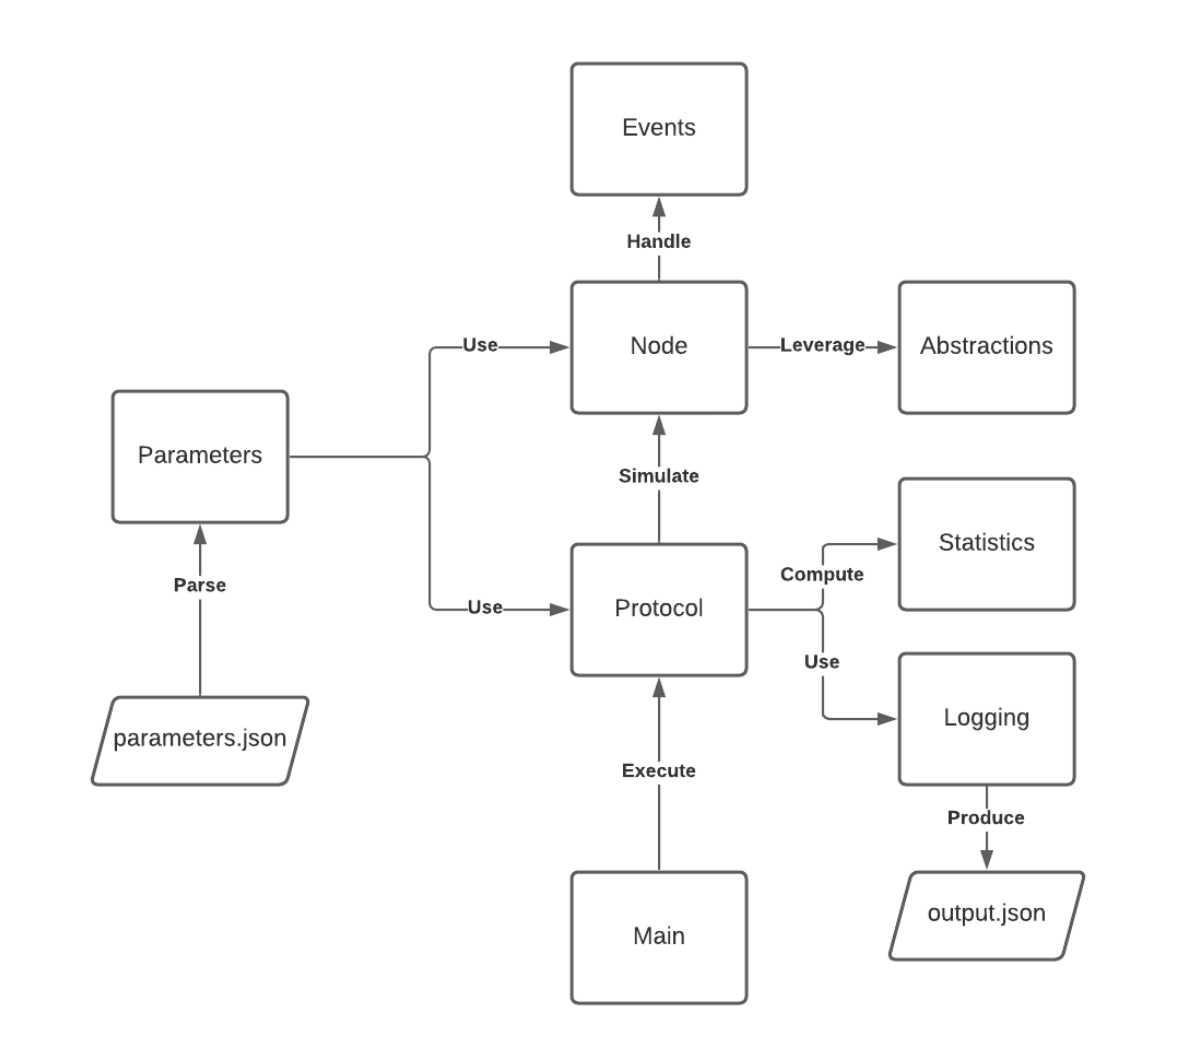
\includegraphics[width=4.5in, angle =0]{modules_mobs}
	\caption{Illustration of top-level module interactions}
	\label{fig:modules_mobs}
\end{figure}

The simulator is built in a module based architecture, Figure~\ref{fig:modules_mobs} illustrates
how the different modules interact. These modules are:
\begin{itemize}
  \item \textbf{Main:} Entry point for the simulator, manages the execution of
protocols.
  \item \textbf{Protocol:} Top-level loop of the simulation, initializes the different
nodes, network topology, event queue and performs event handling and delegation.
  \item \textbf{Node:} This is a user defined module that describes the behaviour
of an entity in the simulated protocol.
  \item \textbf{Abstractions:} This module provides primitives to aid in the
development of new simulation such as proof of stake sortation, proof of work mining,
timers, alarms and message exchanges.
  \item \textbf{Statistics and Logging:}  Extract metrics and values from the execution
to be processed by the GUI.
\end{itemize}

\subsection{Graphical User Interface}\label{subsec:grafical_user_interface}

The graphical user interface was implemented in NodeJS, Vue3 and ElectronJS.
The choice for web technologies enables the future deployment of simulator as
a web application. The GUI was developed with the goal of allowing the users
to use it with their own custom simulators as long as the following conditions are met:

\begin{enumerate}
  \item The simulator uses a parameters.json as an input with three categories,
General, Network and Protocol, the actual parameters inside each category are user defined.
  \item The output of the simulator produces log with two top-level entries, kind and content.
Kind can be one of ten values, each with their specific content, \textit{parameters, 
add-node, add-link, flow-message, add-block, node-committee, node-proposer, create-block,
statistics} and \textit{per-node-statistics}.
\end{enumerate}

The GUI is composed of 4 pages, described in the following sections.

\subsubsection{Parametrization}\label{subsubsec:parametrization}

\begin{figure}[h]
	\centering
	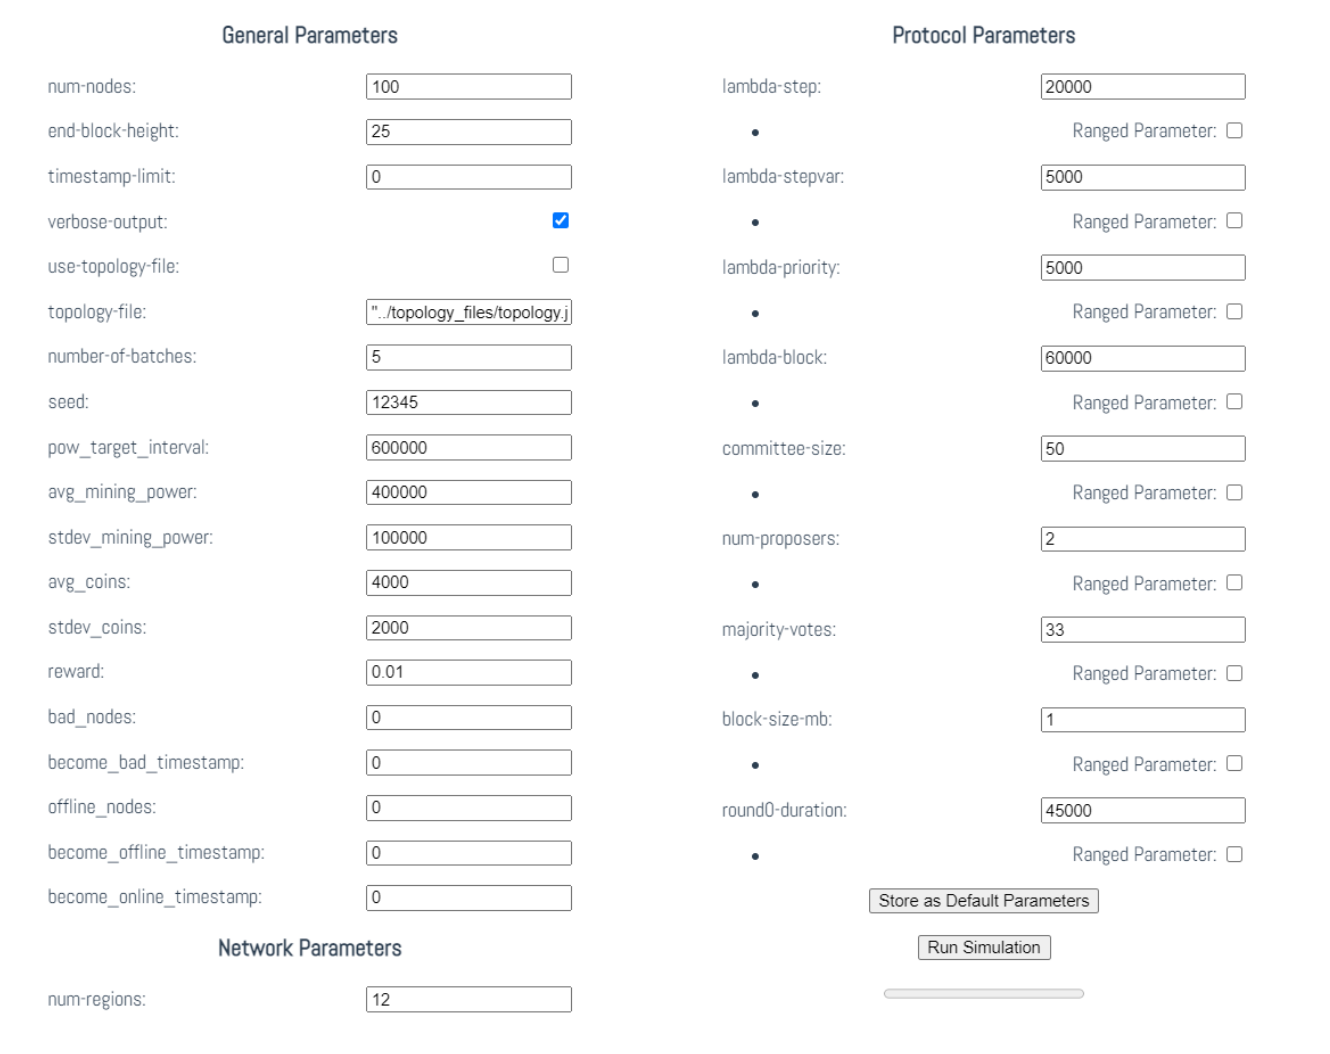
\includegraphics[width=4.5in, angle =0]{mobs_parameters}
	\caption{Parameters window}
	\label{fig:mobs_parameters}
\end{figure}

The Parameters window parses the parameters.json file and produces a form
where the user can customize the values or ranges of values for every parameter.

\subsubsection{Topology Specification}\label{subsubsec:topology_specification}

The GUI also allows user to specify the topology of the network without needing
to manually write the JSON file. The Topology window offers a canvas to construct a network
topology as well as set individual parameters for each node.

\begin{figure}[h]
	\centering
	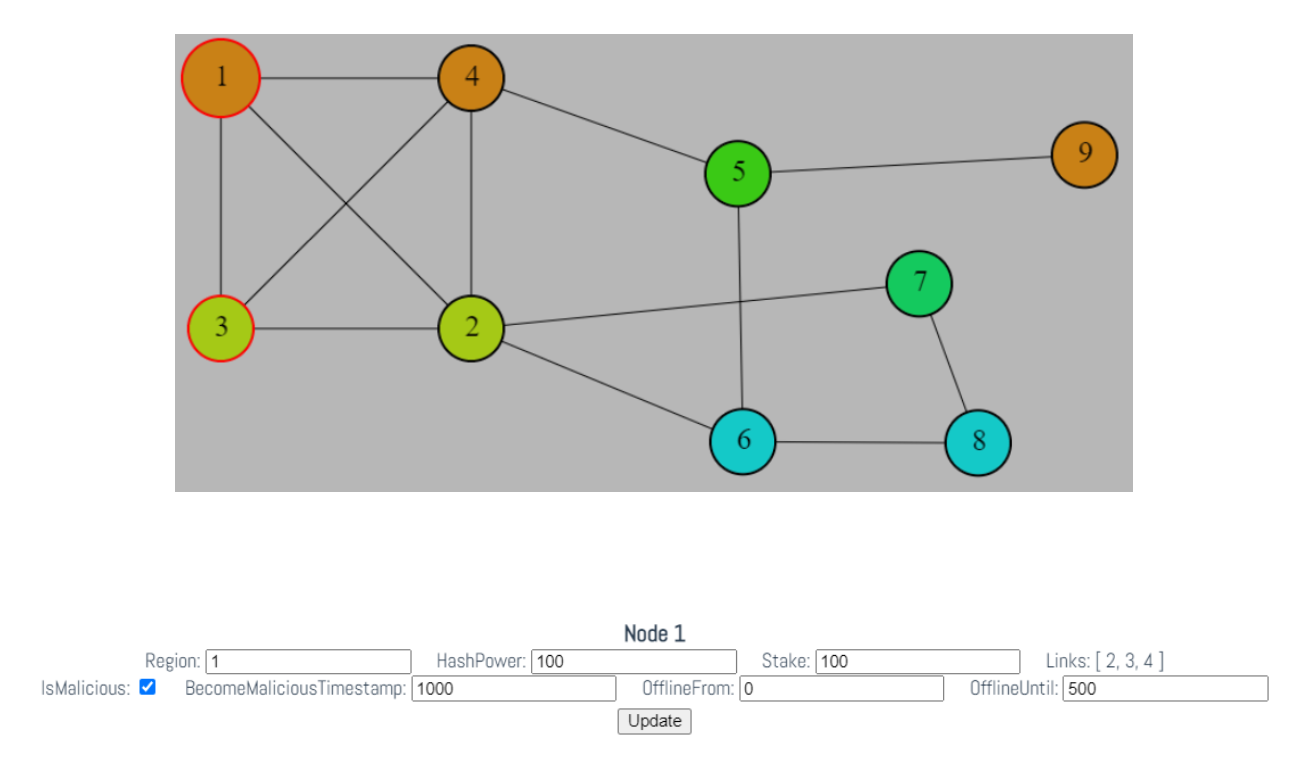
\includegraphics[width=4.5in, angle =0]{topology}
	\caption{Topology window and possible parametrizations for each individual node}
	\label{fig:topology}
\end{figure}

\subsubsection{Visualizer}\label{subsubsec:visualizer}

\begin{figure}[h]
	\centering
	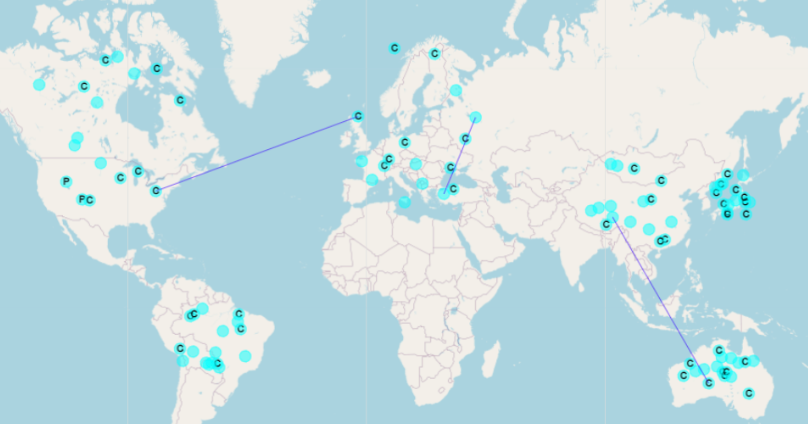
\includegraphics[width=4.5in, angle =0]{visualizer}
	\caption{Time-lapse in the Visualizer window}
	\label{fig:visualizer}
\end{figure}

The Visualizer window allows user to play the state of each node in a time-lapse manner
and visualize exchanged messages.

\subsubsection{Statistical Analysis}\label{subsubsec:statistical_analysis}

The Statistics window aids in the analysis of the metrics produced by the simulator.
The GUI will parse the output.json file and display it in an easy-to-read format.
These formats can come as graphs, displaying minimum and maximum values observed
for each metric that was produced and a graph with per node statistics.

\begin{figure}[h]
	\centering
	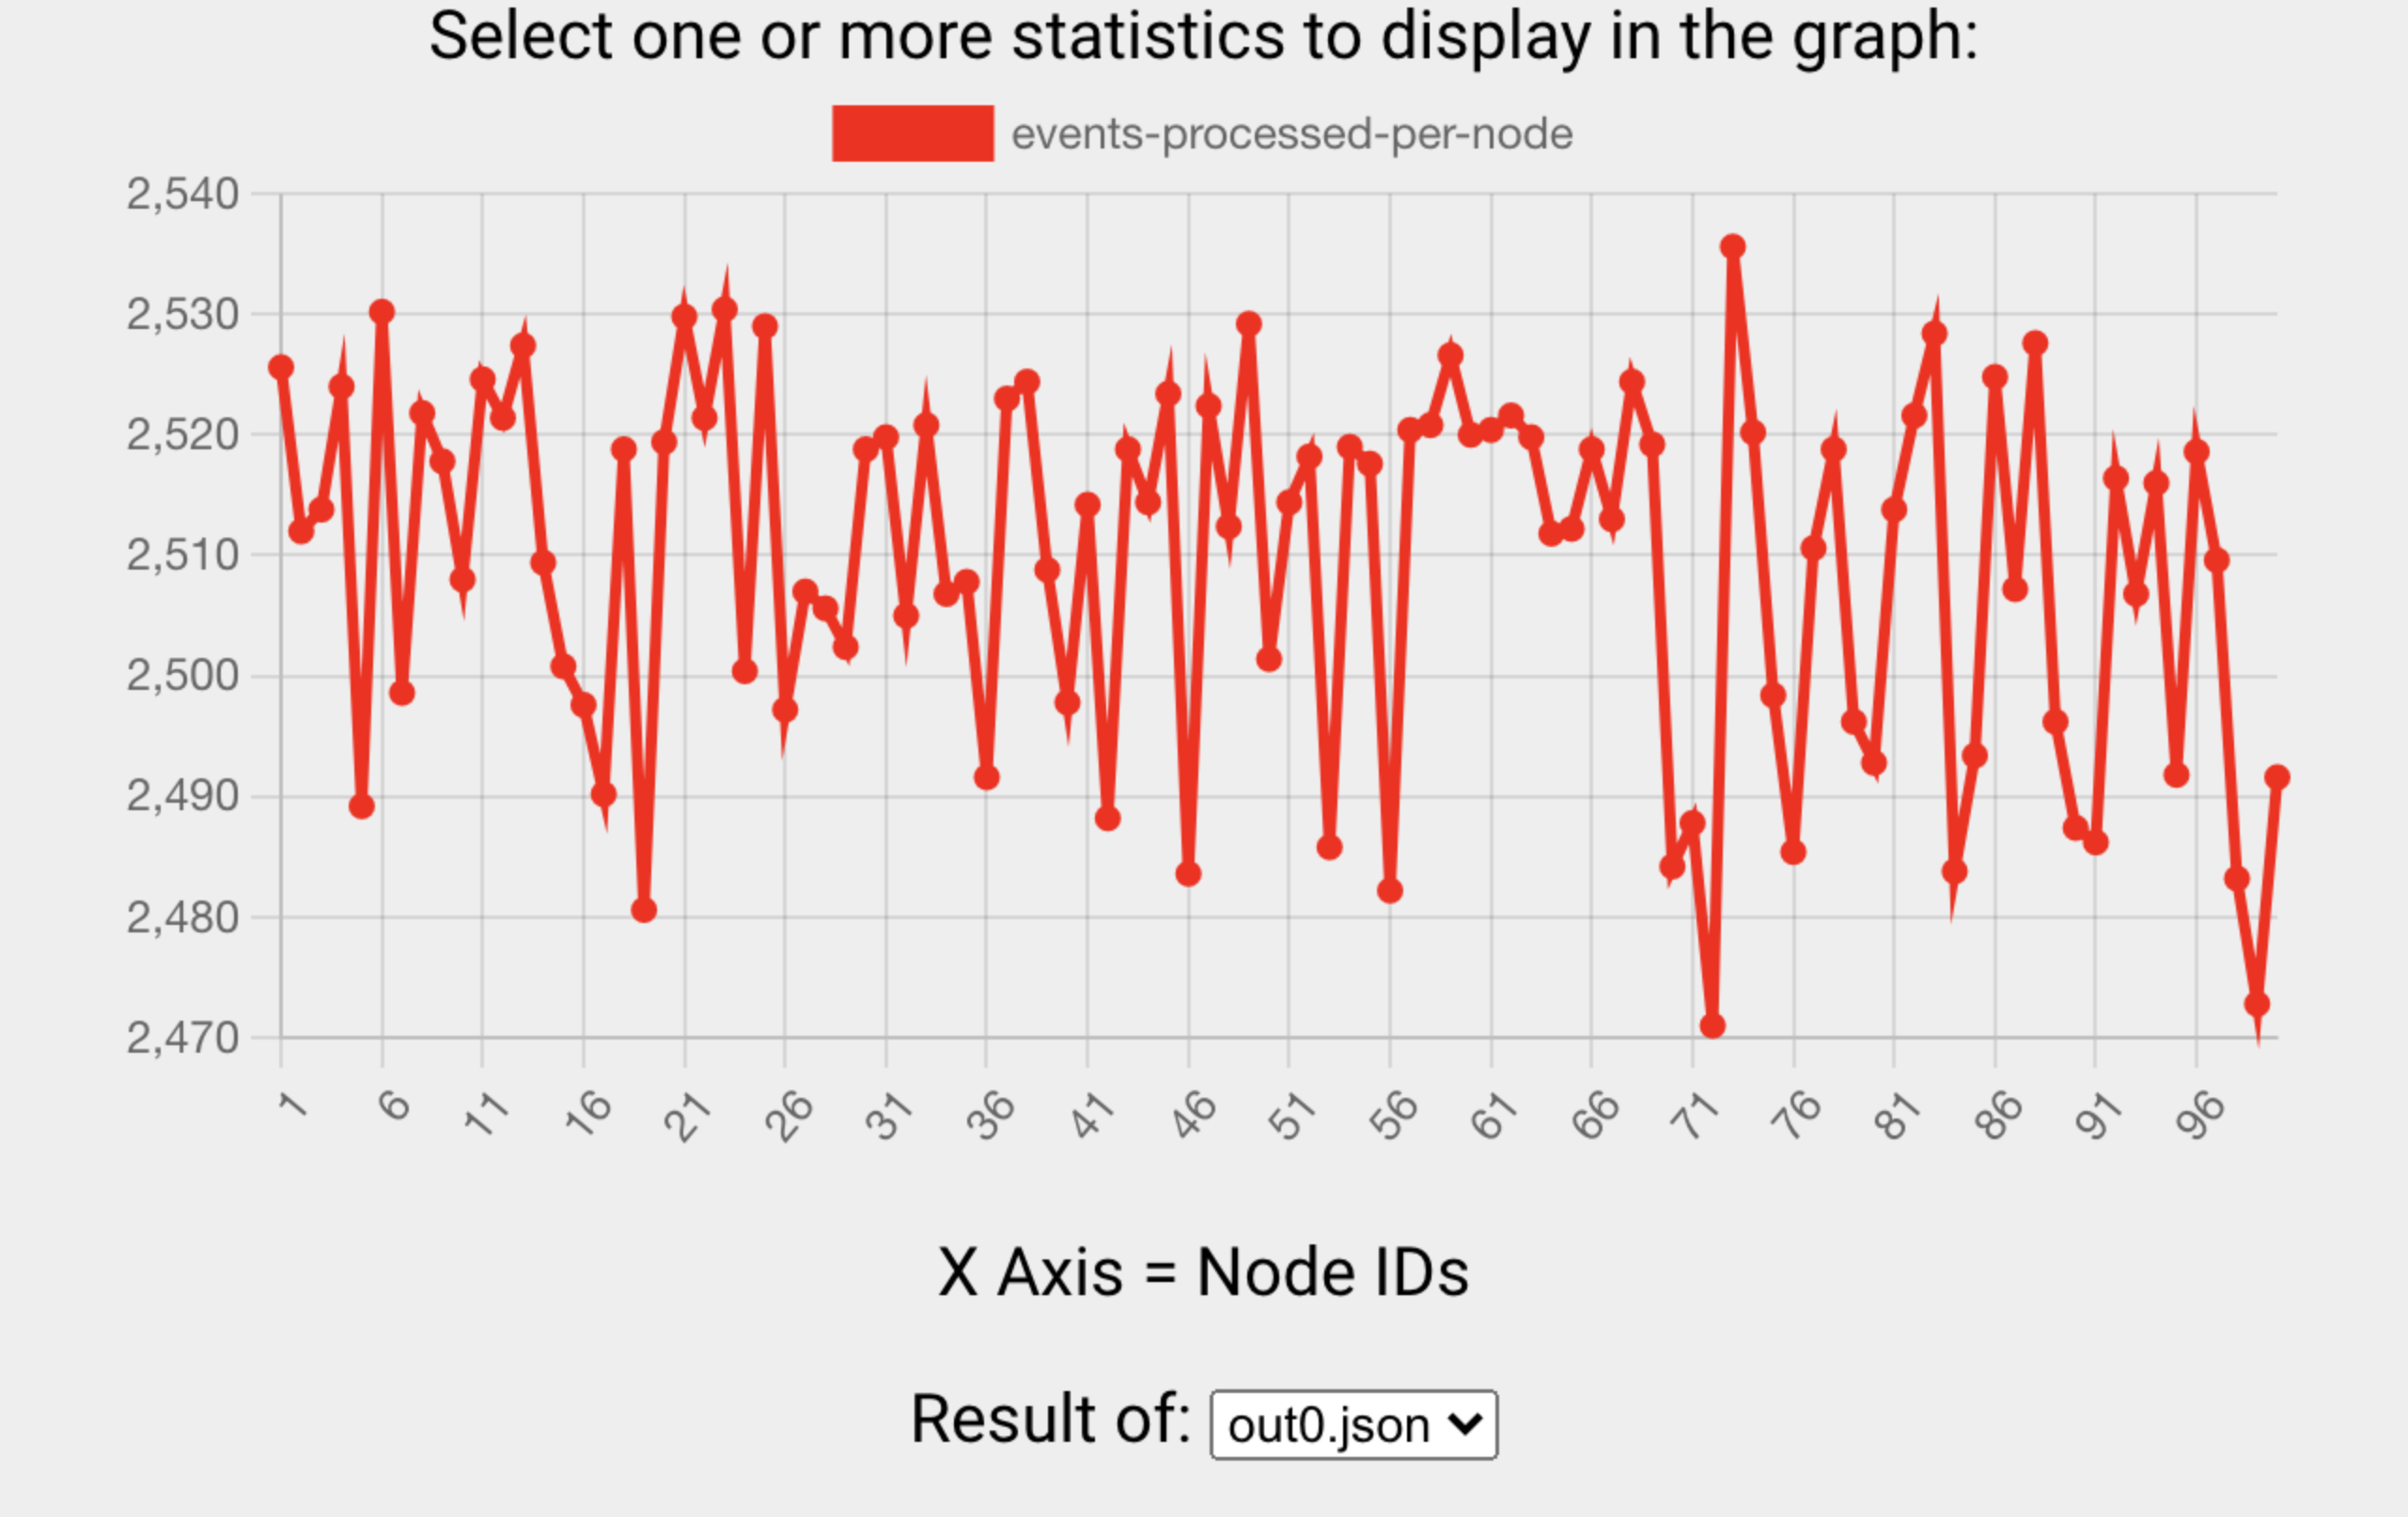
\includegraphics[width=4.5in, angle =0]{statistics}
	\caption{Per Node Statistics window}
	\label{fig:statistics}
\end{figure}

\section{Protocols implemented in MOBS}\label{sub:protocols_implemented_in_mobs}
In this section we describe the implementations we made in MOBS to validate
its capabilities and provide a critical analysis of the process, both with a protocol in
the network layer and several consensus protocols to validate the simulator's capabilities to provide
qualitative metrics through the logs to validate their execution.

\subsection{Chord}\label{sub:chord_implementation}
As an initial exercise we chose to implement Chord in MOBS with the main objective of
evaluating the viability of implementing membership protocols in the network layer. This also
allowed us to better understand the internal structure of MOBS and its limitations.

To achieve this implementation we made use of MOBS Node module and implemented the
following events in accordance to the Chord papper~\cite{chord}:

\begin{itemize}
  \item \textbf{Join: } An event that a node receives when another node first joins
the network. The receiving node will evaluate if the identifier of the new node makes him
a candidate to be that node's predecessor in the ring.
  \item \textbf{JoinResponse: } A node that has previously received a join will reply
with this event if the new node has been accepted as their predecessor. This contains
the identifier of the old predecessor so that the new node can make it its own.
  \item \textbf{Uft: } This event stands for update finger table, this event shares
an identifier known to a node, being from their finger table, their own, or one of
its neighbors with a random node. The receiver node will add this identifier to their finger table.
  \item \textbf{UpdateSuccessor: } This event is only used when a node updates their successor
this event is sent to itself as a way to log the new link.
  \item \textbf{UpdatePredecessor: } This event works the same way as UpdateSuccessor
but for the predecessor node.
  \item \textbf{RebalanceNetwork: } When a node receives this event it comes with
an identifier, the receiver node will see if the identifier is a better candidate for
their successor. This serves as a cyclic membership managing strategy.
  \item \textbf{SendRebalanceNetwork: } Periodically a node will propagate this message
to neighboring nodes to trigger a RebalanceNetwork event with their identifier.
\end{itemize}

These events describe the full execution of the Chord protocol, adapted to a simulator
execution environment providing us with a dynamic membership protocol that provides
a more realistic network layer.

The implementation of this protocol at the Node level turned out to not be successful.

One of the reasons is that when implementing this at the Node module, the network
module implements a network with a random graph, and as an initial operation, one
node would trigger a RebalanceNetwork with the identifier of another node and through
an epidemic broadcast fashion trigger all nodes into trying to join to other nodes.
This resulted in one of two scenarios:

\begin{itemize}
  \item Several Chord rings would be created instead of one single ring with all nodes,
making further communications since at the Chord protocol level, nodes from different rings
would be unknown from each other.
  \item After making nodes send periodic SendRebalanceNetwork events to neighboring
nodes at the Network module level, if the first couple of events made them unable to
integrate the ring they would become dormant, since the trigger to send  new
SendRebalanceNetwork events is triggered  by receiving events from other nodes
\end{itemize}

Another reason this protocol failed was that even leveraging overlay created at
the Network layer to send SendRebalanceNetwork events to know nodes at that level
to ensure that all nodes would converge to the same ring, this would create an enormous
amount of events that would slow down the simulator. This showed some promising results,
and we were able to see signs of a converging network, but the search for better neighbors
at the Chord level turned out to be a blind search, and the closer the network became to
converge the longer it took for new updates to take place.

To solve these issues we proposed move the implementation to the network module level.
This will make possible to initiate one node at a time and reduce blind lookups, solving
all three problems at once: 
\begin{itemize}
  \item Only one ring will be created
  \item Since nodes would always ping a known
member of the ring to join, the protocol would ensure they would be placed on the correct place
of the network and not be left out isolated
  \item Join operations in a formed chord ring would be less costly in the amount
of messages generated since we don't have to broadcast events and can instead target
to specific nodes.
\end{itemize}

We can also leverage this implementation at the network level to make the network
module even more modular and extensible, making it easier to implement new network protocols
and achieving a more dynamic, varied and realistic network layer better mimicing the real world.

\subsection{Consensus protocols}\label{sub:consensus_protocols_implemented}
One of the problems we want to tackle with this thesis is getting better qualitative information out of
blockchain and consensus protocols logs so that we can evaluate their correctness at the end 
of the simulation. To achieve this we implemented three well known consensus protocols
so that we can extract the runtime information and use them as examples to see MOBS' limitations
and if further work needs to be done in Statistics and Logging module.

\subsubsection{Paxos}\label{sub:paxos}

The first of these protocols was Paxos. This was implemented as referenced in~\ref{sub:paxos},
with the only changes to the protocol being based on an optimistic approach such as assuming no malicious nodes
are present in the network, no nodes would fail and no messages would be lost. We also assumed a single proposer
through the entire execution, making this an implementation closer to MultiPaxos
than regular Paxos, this was done for the sake of simplicity an ease of implementation and testing.

To implement this protocol we defined the following events:
\begin{itemize}
	\item \textbf{Propose: } This event is triggered by the proposer node to start a new round, this is used
  as a control message for logging, while the proposer send this to himslf and has no real effect in the protocol,
	it also broadcasts a Prepare message to all its neighbours.
  \item \textbf{Prepare: } This event is broadcasted by the proposer to all nodes to start a new round,
	if the receiving nodes accepts the proposal it will reply with a Promise message to the proposer and
	propagate the Prepare message to its neighbours. This repeats until every node receives the Prepare message
	at least once. If a node detects this message is a duplicate it will ignore it.
  \item \textbf{Promise: } When the proposer receives a Promise message from a node, and it has the same value it was proposed
	it will add the sender to the promise quorum. When the promise quorum reaches over \textit{2/3} of the network size it will
	broadcast an Accept message with the proposed value to all nodes.
  \item \textbf{Accept: } When a node receives an Accept message it will save the value as the decided value and reply
	with an Accepted message to the proposer.
  \item \textbf{Accepted: } The proposer will receive an Accepted message from all nodes that accepted the proposed value,
	when it receives more than \textit{2/3} of the network size it will log the value as accepted and send a Response message
	to itself to log the end of the round. In the real world this would be sent to the client that requested the value to be agreed upon.
  \item \textbf{Response: }	This event is used by the proposer to log the end of a round and the start of a new one.
\end{itemize}

This implies a single and unique proposer throughout the entire execution of the protocol, even though it is possible
to have more than one proposer running at the same time with our implementation.

With the implementation of Paxos done and validated, a script in Python was done that allowed us to
scrub the logs and extract runtime metrics:

\begin{figure}[h]
	\centering
	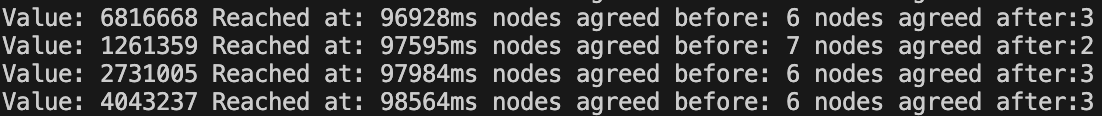
\includegraphics[width=4.5in, angle =0]{consensus_log_script_v1}
	\caption{Output from the first iteration of the log analyser script}
	\label{fig:consensus_log_script_v1}
\end{figure}

This was the first iteration of this script which allowed us to see what value was accepted,
at what tie it was accepted, how many nodes accepted the value and how many accept messages
reached the proposer after the value was accepted. 
On the second iteration of this script we added a section with condensed global data, where we can more
easily observe metrics like number of values accepted, total simulation runtime, average time per consensus
and the average acceptance percentage of consensus.
This script also warns us if there are rounds where more than 1 value was accepted, if a value was
accepted without being proposed or if a value was accepted and the Propose message was sent later than the Accept message.

\begin{figure}[h]
	\centering
	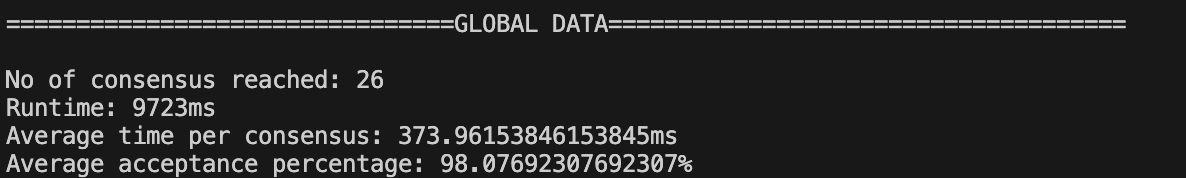
\includegraphics[width=4.5in, angle =0]{consensus_log_script_v2}
	\caption{Output from the second iteration of the log analyser script}
	\label{fig:consensus_log_script_v2}
\end{figure}

The implementation of both the protocol and
the script can be consulted at \href{https://github.com/RMLoureiro/MOBS/pull/2}{this pull request}.

\subsubsection{Chandra-Toueg}\label{sub:chandra-toueg}

We implemented the Chandra-Toueg consensus protocol as described in Section~\ref{sub:chandra-toueg}.
This protocol was selected for its simplicity and compatibility with our simulation framework.
Following the same optimistic approach used for Paxos, we excluded malicious node behavior and
message loss scenarios from the implementation. The logging for this protocol was designed to maintain
compatibility with the analysis script developed for Paxos, enabling the same tool to process
both protocols without modification. The complete implementation details can be found in
\href{https://github.com/RMLoureiro/MOBS/pull/4}{this pull request}.

To implement this protocol we defined the following events:
\begin{itemize}
	\item \textbf{Start: } This event when is received by a node will trigger the start of a new round,
a node will send a Preference message to the coordinator with their proposed value and propagate the Start message
to its neighbours. This repeats until every node receives the Start message at least once. If a node detects
this message is a duplicate it ignores it.
	\item \textbf{Preference: } A preference message is sent by a node to the coordinator with their proposed value,
	when the coordinator receives this message it will add the sender to the preference quorum. When the preference quorum
	reaches over \textit{2/3} of the network size it will broadcast an Accept message with the last proposed value to all nodes.
	\item \textbf{Accept: } When a node receives an Accept message it will save the decided value and reply
	with an Ack message to the coordinator while propagating the Accept message through gossip.
	\item \textbf{Ack: } The coordinators receive an Ack message from each proposer confirming they accepted the proposed value,
	when it receives more than \textit{2/3} of the network size it will log the value as accepted and send a Consensus message
	to itself to log the end of the round. In the real world this would be sent to the client that requested the value to be agreed upon.
	\item \textbf{Consensus: }	This event is used by the proposer to log the end of a round and the start of a new one.
\end{itemize}

When we completed our implementation we validated it using the same script used for Paxos,
we found that the script was able to parse the logs without any modifications, we found that
the protocol was able to reach consensus in all rounds and the metrics extracted indicated that
Chandra-Toueg took on average half the time Paxos took to reach consensus.

\begin{figure}[h]
	\centering
	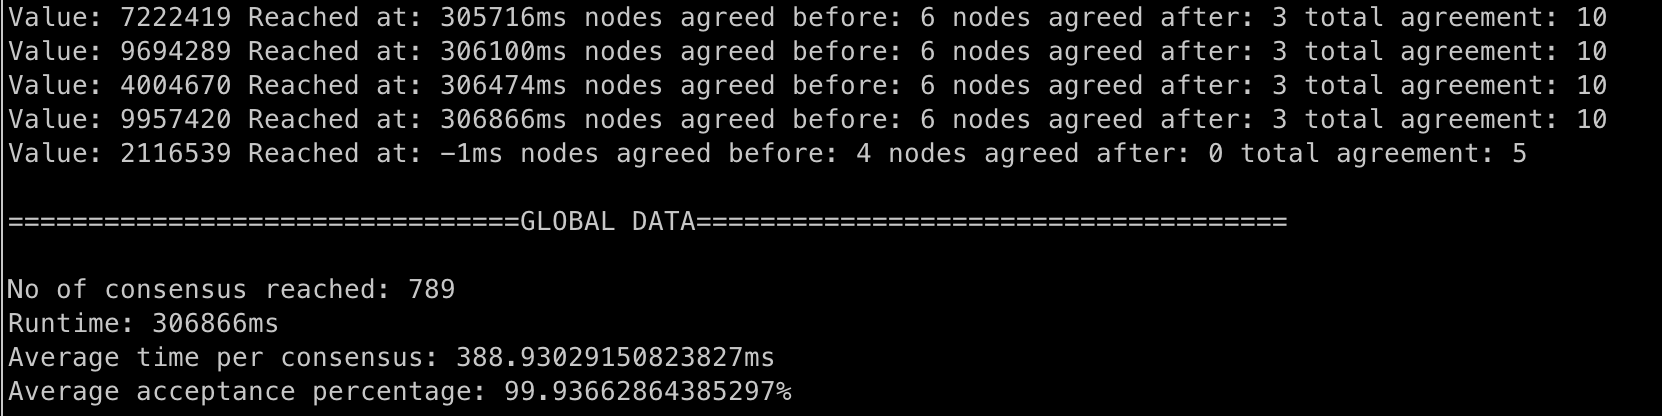
\includegraphics[width=4.5in, angle =0]{chandra-toueg-metrics}
	\caption{Output from the log analyser script for a Chandra-Toueg execution}
	\label{fig:chandra-toueg-metrics}
\end{figure}

\subsubsection{Practical Byzantine Fault Tolerance}\label{sub:practical_byzantine_fault_tolerance}

The last protocol of the consensus family we implemented Practical Byzantine Fault Tolerance (PBFT) as described
in~\ref{sub:pbft}, we chose this protocol for its robustness and ability to handle malicious nodes.
We again focused on an optimistic implementation where we didn't take into account lost messages.
The implementation can be consulted at \href{https://github.com/RMLoureiro/MOBS/pull/6}{this pull request}.

To achieve this implementation we implemented the following events:
\begin{itemize}
	\item \textbf{Request: } This event is sent to the client node to start a new round, this is used
	as a control message for logging, the client will gossip a Pre-Prepare message to all its neighbours.
	\item \textbf{Pre-Prepare: } All other nodes do their startup with this message,
	when the receiving nodes accepts the proposal it will send with a Prepare message to all the other nodes.
	\item \textbf{Prepare: } When receiving a Prepare message  the receiver
	adds the node to the prepare quorum if the value matches the proposed one.
	When the prepare quorum reaches over \textit{2/3} of the network size it will
	broadcast a Commit message with the proposed value to all nodes.
	\item \textbf{Commit: } When a node receives a Commit message it will save the value as the decided value and it saves
	the sender in a commit quorum. When the commit quorum reaches over \textit{2/3} of the network size it will
	reply with a Reply message to the client.
	\item \textbf{Reply: } The client will receive a Reply message from all nodes that accepted the proposed value,
	when it receives more than \textit{2/3} of the network size send itself an Accept message for logging purposes, marking the end of
	the current round.
	\item \textbf{Accept: } This is just a logging event used by the client to log the end of a round, to start the next round
	it will send a random node in the network a Request message, selecting a new leader for the next round.
	\item \textbf{ViewChange: }	The view change mechanism prevents nodes from being stuck waiting for messages from a faulty client,
  In the real world this timeout would trigger a client change, but in our optimistic implementation we just increment the view number
	and send a New View message to the client.
	\item \textbf{NewView: } This message is sent to the client by all other nodes to inform them of the new view number. When a message
	is received the client saves the senders in a new view quorum, when this quorum reaches over \textit{2/3} of the network size
	it will send a ApplyNewView message to all nodes so that they can start a new view.
	\item \textbf{ApplyNewView: } When a node receives a New View message, it will update its view number.
\end{itemize}

There is also an implementation of a script to validate the logs like we did for Paxos and Chandra-Toueg,
that allowed us to validate the protocol and extract metrics like the number of consensus reached,
average time per consensus and average acceptance percentage. This script also shows how many times each client
got its values approved.
The script is also able to detect when there are no values accepted, which can happen if the view change
mechanism is triggered too often, preventing the protocol from reaching consensus. This warning is issued if there
are more than 5 view changes without a value being accepted.

\begin{figure}[h]
	\centering
	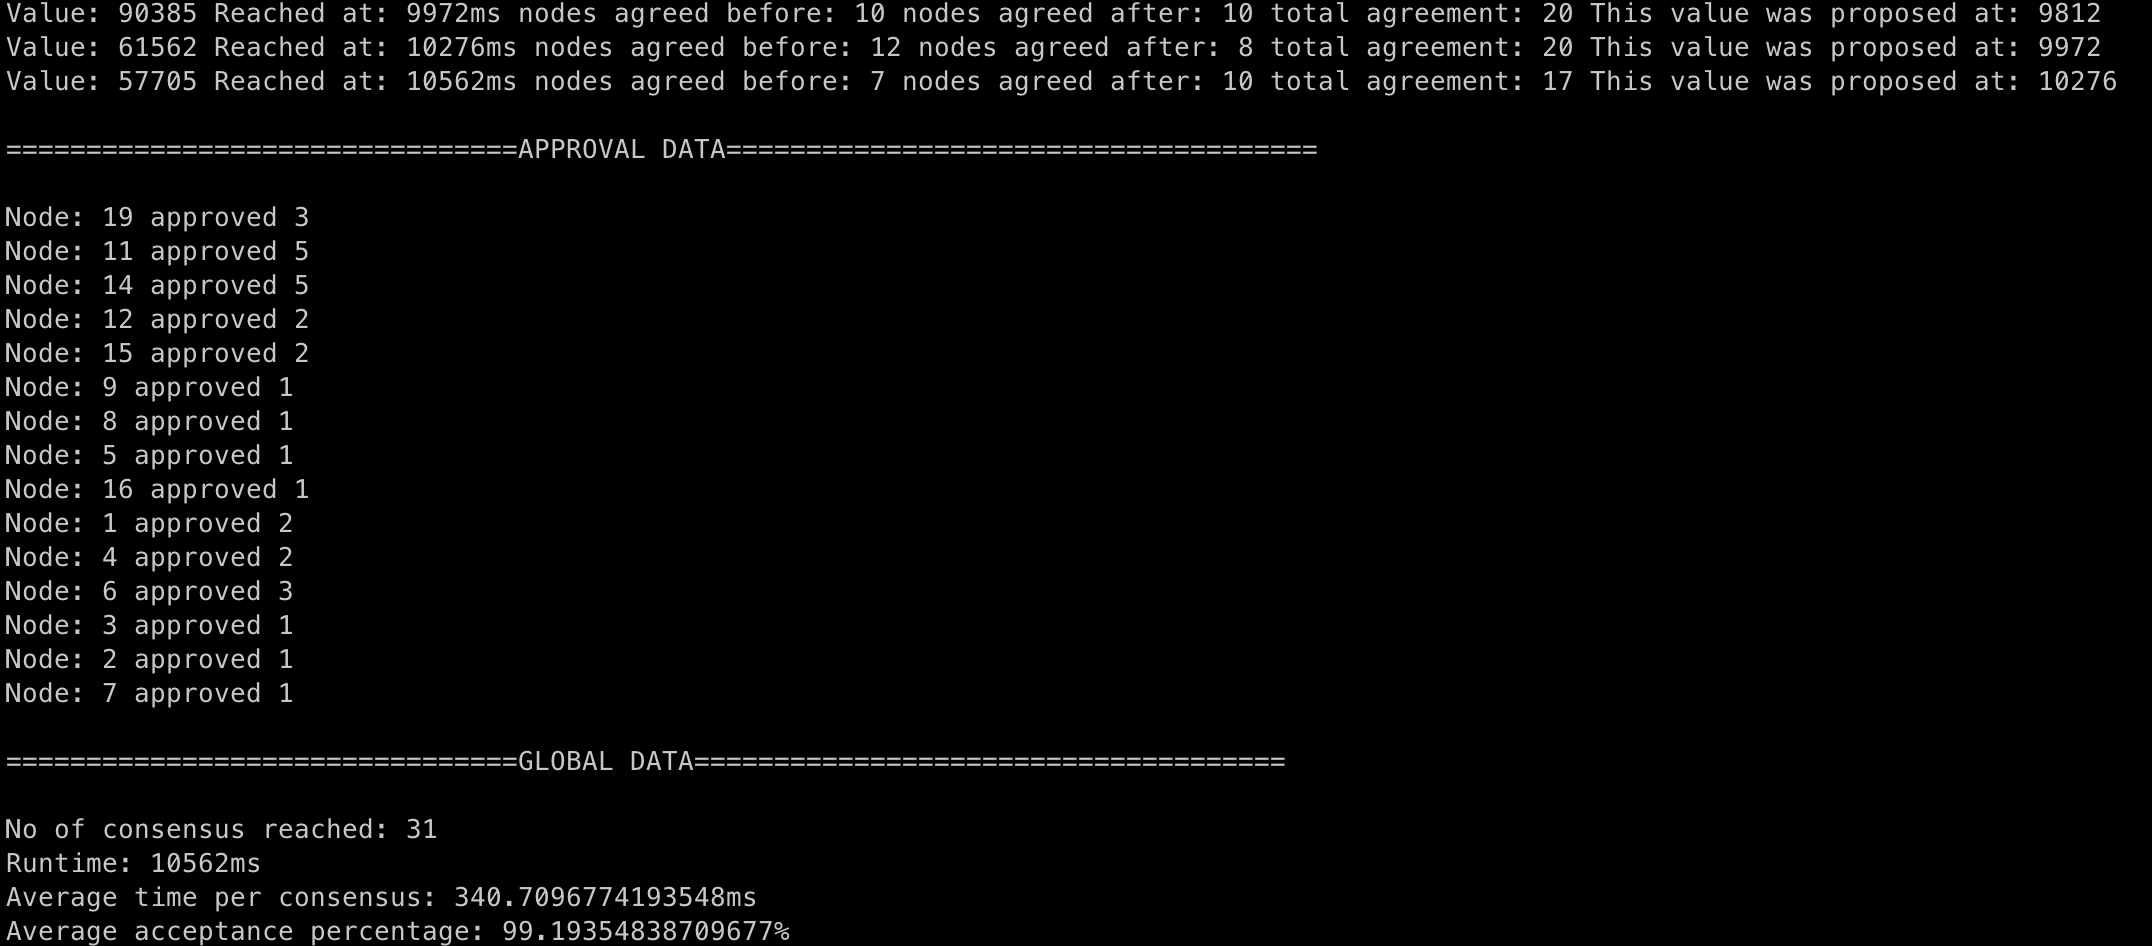
\includegraphics[width=4.5in, angle =0]{pbft_metrics}
	\caption{Output from the log analyser script for a pBFT execution}
	\label{fig:pbft_metrics}
\end{figure}

\subsubsection{Results Analysis}\label{sub:results_comparison}
After the implementations were completed we compared their executions.
For all executions we ran for a simulated time o 1.000.000ms with a network of 20 nodes and extracted
the following metrics: average time per consensus, average acceptance percentage and number of consensus reached.
The results can be seen in Table~\ref{tab:simulation_comparison}.


\begin{table}[h]
	\caption{Average results from 20 executions at 10000ms runtime}\label{tab:simulation_comparison}
	\begin{tabular}{|c|c|c|c|}
	\hline
						   & \textbf{\begin{tabular}[c]{@{}c@{}}Average Time \\ per Consensus\end{tabular}} & \textbf{\begin{tabular}[c]{@{}c@{}}Average acceptance \\ percentage\end{tabular}} & \textbf{\begin{tabular}[c]{@{}c@{}}Number of \\ consensus reached\end{tabular}} \\ \hline
	\textbf{Paxos - 1 Proposer}         & 289.46 ms                                                                      & 99.12\%                                                                           & 3454                                                                              \\ \hline
	\textbf{Paxos - Multiple Proposers}         & 525.09 ms                                                                      & 99.35\%                                                                           & 1278                                                                              \\ \hline
	\textbf{Chandra-Toueg} & 188.10ms                                                                      & 99.99\%                                                                           & 5316                                                                              \\ \hline
	\textbf{pBFT} & 304.58ms                                                                      & 98.63\%                                                                           & 3283                                                                              \\ \hline
	\end{tabular}
\end{table}

Paxos with a single proposer was
significantly faster than with multiple proposers, which is expected since multiple proposers
can create conflicts and increase the time to reach consensus. Chandra-Toueg was the fastest protocol,
which aligns with its design for efficiency in asynchronous systems. PBFT, while robust against Byzantine faults,
was slower than Paxos with a single proposer but faster than Paxos with multiple proposers.
We found that all protocols had a high acceptance percentage, and even though we were expecting 100\%
acceptance in all protocols,
after manually analysing the logs we came to the conclusion that the missing percentage of acceptance
came from the protocol runtime being limited and the simulation ending before all the Accept
messages reached the proposer, since all values before accounted for 100\% acceptance.